\documentclass[a4paper,10pt,twoside]{article}

\usepackage[top=1in, bottom=1in, left=1in, right=1in]{geometry}
\usepackage[utf8]{inputenc}
\usepackage[spanish,es-ucroman,es-noquoting]{babel}
\usepackage{setspace}
\usepackage{fancyhdr}
\usepackage{lastpage}
\usepackage{amsmath}
\usepackage{amsfonts}
\usepackage{verbatim}
\usepackage{graphicx}
\usepackage{float}
\usepackage{algorithmic}
\usepackage{tikz}
\usetikzlibrary{calc}
\usetikzlibrary{decorations.pathreplacing}


% Evita que el documento se estire verticalmente para ocupar
% el espacio vacío en cada página.
\raggedbottom

\newenvironment{pseudocodigo}
    {\vspace{0.5em} \begin{algorithmic}}
    {\end{algorithmic} \vspace{0.5em}}


%%%%%%%%%% Configuración de Fancyhdr - Inicio %%%%%%%%%%
\pagestyle{fancy}
\thispagestyle{fancy}
\lhead{Trabajo Práctico 2, Organización del Computador II}
\rhead{Belloli, Lovisolo, Petaccio}
\renewcommand{\footrulewidth}{0.4pt}
\cfoot{\thepage /\pageref{LastPage}}

\fancypagestyle{caratula} {
   \fancyhf{}
   \cfoot{\thepage /\pageref{LastPage}}
   \renewcommand{\headrulewidth}{0pt}
   \renewcommand{\footrulewidth}{0pt}
}
%%%%%%%%%% Configuración de Fancyhdr - Fin %%%%%%%%%%


\begin{document}


%%%%%%%%%%%%%%%%%%%%%%%%%%%%%%%%%%%%%%%%%%%%%%%%%%%%%%%%%%%%%%%%%%%%%%%%%%%%%%%
%% Carátula                                                                  %%
%%%%%%%%%%%%%%%%%%%%%%%%%%%%%%%%%%%%%%%%%%%%%%%%%%%%%%%%%%%%%%%%%%%%%%%%%%%%%%%


\thispagestyle{caratula}

\begin{center}


\includegraphics[height=2cm]{DC.png} 
\hfill

\includegraphics[height=2cm]{UBA.jpg} 

\vspace{2cm}

Departamento de Computación,\\
Facultad de Ciencias Exactas y Naturales,\\
Universidad de Buenos Aires

\vspace{4cm}

\begin{Huge}
Trabajo Práctico 3
\end{Huge}

\vspace{0.5cm}

\begin{Large}
Organización del Computador II
\end{Large}

\vspace{1cm}

Primer Cuatrimestre de 2013

\vspace{4cm}

Grupo: \textbf{Panceta y Mozzarella}

\vspace{0.5cm}

\begin{tabular}{|c|c|c|}
\hline
Apellido y Nombre & LU & E-mail\\
\hline
Laouen Louan Mayal Belloli  & 134/11 & lao.facu@gmail.com\\
Leandro Lovisolo      		& 645/11 & leandro@leandro.me\\
Lautaro José Petaccio 		& 443/11 & lausuper@gmail.com\\
\hline
\end{tabular}

\end{center}

\newpage


%%%%%%%%%%%%%%%%%%%%%%%%%%%%%%%%%%%%%%%%%%%%%%%%%%%%%%%%%%%%%%%%%%%%%%%%%%%%%%%
%% Índice                                                                    %%
%%%%%%%%%%%%%%%%%%%%%%%%%%%%%%%%%%%%%%%%%%%%%%%%%%%%%%%%%%%%%%%%%%%%%%%%%%%%%%%


\tableofcontents

\newpage


%%%%%%%%%%%%%%%%%%%%%%%%%%%%%%%%%%%%%%%%%%%%%%%%%%%%%%%%%%%%%%%%%%%%%%%%%%%%%%%
%% Introducción                                                              %%
%%%%%%%%%%%%%%%%%%%%%%%%%%%%%%%%%%%%%%%%%%%%%%%%%%%%%%%%%%%%%%%%%%%%%%%%%%%%%%%


\section{Introducción}

bla bla bla

\section{Desarrollo}
\subsection{Ejercicio 1: GDT y modo protegido}
\subsubsection{Completando la tabla de descriptores de segmento GDT}
Teniendo en cuenta el manual de intel, la primer entrada de la GDT debe ser nula, por lo que la misma fue llenada toda con $0$.
Además tenemos que crear $6$ entradas, $3$ para códigos de nivel $0$, $2$ y $3$, y $3$ para datos de nivel $0$, $2$ y $3$. 

Como estamos definiendo nuestro SO con un sistema Flat, todas las bases de los $6$ segmentos mensionados son $0$. y su limite es $0x7FFFF$ lo cual nos da un espacio de memoria de $2GB$ pedidos en el enunciado del TP. \\

A continuación se enuncia detalladamente como fueron cargados los descriptores. \\

\textbf{Segmento 1: ( segmento de código )}
\begin{itemize}
 \item $limit\_0\_15 = 0xFFFF$ (Se encuentran los primeros $16$ bits que indican el limite del segmento, poniendo este valor, como la base es $0$ obtenemos segmentos de $2GB$ como fue pedido en el enunciado del TP).
 \item $base\_0\_15 = 0$ 
 \item $base\_23\_16 = 0$
 \item $type = 10$ (Para segmentos correspondientes a código el tipo debe ser $10$ = $1010$).
 \item $s = 1$ 	(Este bit en $1$ indica que el segmento no pertenece al sistema).
 \item $dpl = 0$ (En este bit declaramos que privilegios tiene el segmento).
 \item $p = 1$ (Seteando en $1$ este bit indicamos que el segmento está presente en la memoria.).
 \item $limit\_16\_19 = 0x7$ (acá están los últimos $4$ bits del limite).
 \item $avl = 0$
 \item $l = 0$ (como no trabajamos en modo $IA-32e$ debe estar en $0$).
 \item $db = 1$
 \item $g = 1$ (Esto indica la unidad de medida del campo límite. Estando en $1$ indica que cada unidad es de $4kb$).
 \item $base\_31\_24  = 0$
\end{itemize}

\textbf{Segmento $2$: ( segmento de código )} \\
Es muy similar al segmento $1$ solo que cambia el nivel de privilegio definido en $dpl$ que pasa a ser $1$. \\

\textbf{Segmento $3$: ( segmento de código )} \\
Es muy similar al segmento $1$ solo que cambia el nivel de privilegio definido en $dpl$ que pasa a ser $2$. \\

\textbf{Segmento $4$: ( segmento de datos )} \\
Es muy similar al segmento $1$ cambiando el atributo $type$ por $2$ = $0010$. \\

\textbf{Segmento $5$: ( segmento de datos )} \\
Es muy similar al segmento anterior solo que cambia el nivel de privilegio definido en $dpl$ que pasa a ser $1$. \\

\textbf{Segmento $6$: ( segmento de datos )} \\
Es muy similar al segmento anterior solo que cambia es el nivel de privilegio definido en $dpl$ que pasa a ser $2$. \\ 

Además de esto hay que declarar un segmento de datos más para describir el área de la pantalla en memoria, el mismo esta definido de la siguiente manera: 
\begin{itemize}
 \item $limit\_0\_15 = 0x7FFF$
 \item $base\_0\_15 = 0x8000$ 
 \item $base\_23\_16 = 0xB$
 \item $type = 2$
 \item $s = 1$
 \item $dpl = 3$
 \item $p = 1$
 \item $limit_16_19 = 0$
 \item $avl = 0$
 \item $l = 0$
 \item $db = 1$
 \item $g = 0$
 \item $base\_31\_24  = 0$
\end{itemize}

Si observamos veremos que la base es $0xB8000$ (dirección de memoria donde empieza la memoria de video), el limite es $0x07FFF$ (el límite de la memoria de video es $0xC0000$ por lo tanto $0xC0000-1 = 0x07FFF$) y su granularidad es 0 ya que su límite puede determinar la memoria necesaria sin usar granularidad. (VER TP TIENE GRANULARIDAD 1 ERROR CREO)

\subsubsection{Pasando a modo protegido}

A continuación veremos el codigo que pasa de modo real a modo protegido.

\begin{pseudocodigo}
  \STATE
  \STATE \textbf{(Desabilitando las interrupciones)}
  \STATE cli
  \STATE
  \STATE call habilitar\_A20
  \STATE
  \STATE \textbf{(carga la GDT definida anteriormente)}
  \STATE lgdt [GDT\_DESC]
  \STATE
  \STATE \textbf{(setea el bit PE del registro CR0)}
  \STATE mov eax, cr0
  \STATE or eax, 1
  \STATE mov cr0, eax
  \STATE
  \STATE \textbf{(pasa a modo protegido, segmento 8 es código nivel 0)}
  \STATE jmp 0x8:modo\_protegido
  \STATE BITS 32
  \STATE cli
  \STATE 
  \STATE \textbf{( setear los segmentos )}
  \STATE mov ax, 32
  \STATE mov ss, ax
  \STATE mov ds, ax
  \STATE mov es, ax
  \STATE mov gs, ax
  \STATE mov ax, 56
  \STATE mov fs, ax
  \STATE 
  \STATE \textbf{( setea la pila )}
  \STATE mov EBP, 0x00020000	
  \STATE mov ESP, 0x00020000
\end{pseudocodigo}

la función $habilitar\_A20$ creada por la catedra sirve para poder extender la limitación inicial de 20 lineas de direccionamiento a 32. La misma debe ser llamada antes de pasar al modo protegido, ya que si no se genera un general protection $\#GP$.

También se debe cargar la GDT, ya que una vez que pasemos a modo protegido se empezará a utilizar la misma para gestionar la memoria. Es por esto que las primeras acciones que se llevan a cabo luego de pasar a modo protegido es setear los selectores de segmento correctamente y pasarle la dirección de la pila a los registros \textbf{EBP} y \textbf{ESP}. Si esto no se llevara a cabo rapidamente, se corre el riezgo de tener errores, ya que si se necesitace usar estos recursos, los mismos estarían con basura.

\subsection{Ejercicio 2: Completar la IDT}
La IDT (Interrupt Descriptor Table) es la encargada de almacenar los descriptores de interrupciones, la misma tiene un total de 256 entradas, las cuales se corresponden con todos los distintos tipos de interrupciones que maneja el microprocesador, estas pueden ser excepciones o interrupciones provocadas por el usuario. Las entradas 2, 15 y de la 20 a la 31 están reservadas por intel, por lo que no hay que utilizarlas. Para el resto de las entradas, se creó en $isr.asm$ la rutina de atención correspondiente y se llenó con los descriptores correctos para que apunten a la rutina creada.
Para llenar la IDT con sus descriptores utilizamos el archivo $idt.c$, el cual contiene la siguiente macro creada por la cátedra que facilita el trabajo del mismo.\\

\#define IDT\_ENTRY(numero, seg, atrr) \\                                                                      
\ \ \ \ idt[numero].offset\_0\_15 = (unsigned short) ((unsigned int)(\&\_isr \#\# numero) \& (unsigned int) 0xFFFF); \\
\ \ \ \ idt[numero].segsel = (unsigned short) seg; \\
\ \ \ \ idt[numero].attr = (unsigned short) atrr; \\
\ \ \ \ idt[numero].offset\_16\_31 = (unsigned short) ((unsigned int)(\&\_isr \#\# numero) $>>$ 16 \& (unsigned int) 0xFFFF); \\

En $numero$ va la posición de la IDT correspondiente a la entrada, en $seg$ el segmento que utilizara y en $atrr$ los atributos correctos.

Estos atributos deben ser seteados teniendo en cuenta los atributos correctos.

\subsubsection{atributos}

A continuación mostramos la lista de atributos que explicaremos.
\begin{itemize}
 \item $p$
 \item $dpl$
 \item $s$
 \item $d$
 \item $tipo$ $de$ $descriptor$ $(3$ $bits)$
 \item $3$ $bits$ $en$ $0$
\end{itemize}

El primer bit $p$ es el que indica que la interrupcion está presente en memoria.

$dpl$ hace referencia a los privilegios que necesita el proceso para poder llamar a la rutina. Un proceso que tiene privilegio de usuario ($3$) no puede llamar a una rutina que tiene $dpl = 0$ ya que el mismo indica que solo un proceso con privilegio de kernel puede llamarlo.

Además como lo que queremos definir son puertas de interrupcion, hay que definir como $1 1 0$ los 3 bits de $tipo$ $de$ $descriptor$.

Los siguientes 3 bit deben ser seteados en $0$ ya que asi lo indica el manual de intel.\\

Teniendo estas cosas en cuenta, los tres números en hexadecimal que se le pasa al campo $atrr$ para definir las entradas correctamente son:

\begin{enumerate}
 \item $0x8E00 = | 1 | 0 0 | 0 1 1 1 0 | 0 0 0 | 0 0 0 0 0 | $ \\ aqui definimos los atributos para rutinas con nivel de privilegios de kernel.
 \item $0xCE00 = | 1 | 1 0 | 0 1 1 1 0 | 0 0 0 | 0 0 0 0 0 | $ \\ aqui definimos los atributos para rutinas con nivel de privilegios $2$.
 \item $0xEE00 = | 1 | 1 1 | 0 1 1 1 0 | 0 0 0 | 0 0 0 0 0 | $ \\ aqui definimos los atributos para rutinas con nivel de privilegios de usuario.
\end{enumerate}

Luego utilizando esto, llenamos todos los campos necesarios en la IDT correctamente. Todas las excepciones utilizarán el segmento de código del kernel salvo las interrupciones $0x80$ y $0x90$, las cuales tienen nivel de privilegio $3$ y $2$ respectivamente que servirán para permitir a los usuarios y al árbitro utilizar los servicios del kernel.


\subsection{Ejercicio 3: inicializar el directorio y las tablas de paginas del kernel}
\subsubsection{Inicializando page\_directory}
Para poder activar paginación primero debemos inicializar el page directory y los page table tanto del kernel como de las tareas. Teniendo en cuenta que la cantida de espacio que necesita el kernel es de $1.39$ MB alcanza con definir un solo page table para mapear todo este espacio.

Es por esto que utilizando la siguiente rutina inicializamos primero todas las entradas del page directory del kernel en $0$.

\begin{pseudocodigo}
  \STATE pd\_entry\* page\_directory = (pd\_entry\*) KERNEL\_PAGE\_DIR
  \STATE int i;
  \FOR {$i = 0; i < 1024; i++$} 
    \STATE \*((unsigned int\*) \&(page\_directory[i])) = 0;
  \ENDFOR
\end{pseudocodigo}

El siguiente paso es definir correctamente la primer entrada, la cual está ubicada en page\_directory[0].

Para hacer esto hay que tener en cuenta como asignar los atributos. 

\begin{itemize}
 \item $user\_supervisor = 0$;
 \item $address = KERNEL\_PAGE\_TABLE >> 12$;
 \item $read_write = 1$;
 \item $present = 1$;
\end{itemize}

De esta manera indicamos que esa página tiene privilegios de supervisor ($user\_supervisor$ en 0), además dice en que parte de la memoria fisica esta alojada la page table, que la misma es de lectura y escritura y que está presente en la memoria.
Como mencionamos antes, basta cargar estos datos en la primer entrada del page directory para mapear todo el espacio necesario para el kernel del TP.

\subsubsection{inicializando page\_table}
Una vez que esta definido el page directory, debemos inicializar correctamente las entradas del page\_table[0] que definimos anteriormente.

Hay que direccionar un espacio de $1.39$ MB =  $1424$ Kb lo cual entra en $356 = 0x164$ paginas de $4$ Kb. Teniendo en cuenta que la cantidad de entradas de un page table es de $1024$ setearemos las todas las entradas en $0$ con una rutina idéntica a la utilizada en el page directory y luego las primeras $356$ las re-seteamos corréctamente.

Las entradas del page table tienen la misma estructura que el page directory, y como lo que tenemos que hacer es $identity$ $mapping$, lo que necesitamos es que dada una dirección virtual $A$, esta corresponda a la misma dirección física. Para esto en el campo $adress$ le ponemos el mismo número de la page entry que estamos seteando para determinar que la misma página virtual se corresponde con la misma física.

$page\_table[i].adress = i$

Tengamos en cuenta como se decodifica la dirección virtual para obtener una dirección fisica. La misma se puede dividir en $3$ segmentos.

\begin{enumerate}
 \item directorio = contiene el offset dentro del page directory donde se encuentra la page table correspondiente.
 \item tabla = este es el offset dentro del page table donde se encuentra el descriptor de la página correspondiente.
 \item Offset = este es el offset que se le suma a la base de la pagina obtenida para obtener el espacio de memoria exacto que queremos
\end{enumerate}

Como la unica entrada del page directory que utilizaremos es la $0$, el campo directorio deberá ser siempre $0$, lo cual es correcto ya que los últimos $10$ bits de cualquier dirección del kernel son $0$. Luego dentro del page table obtenemos la dirección base de la página, la cual se obtiene de buscar la tabla indicada por el campo table (los bits 12 a 21 de la dirección virtual). Al definirle adress con el mismo número al de la entrada de esa tabla, al momento de sumar el offset de la dirección, obtendremos claramente un $identity$ $mapping$. \\

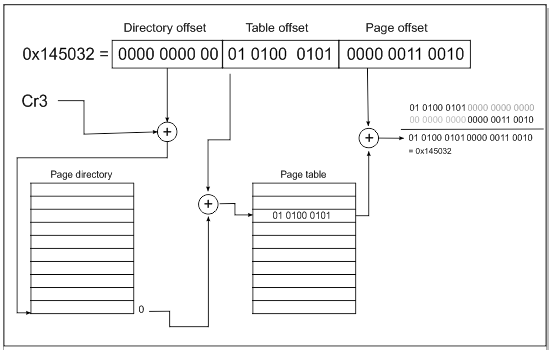
\includegraphics[height=7cm]{iddMap.png}

\subsection{Ejercicio 4: inicializar el directorio y las tablas de paginas}

Para el caso de las tareas lo que sucede es similar, a diferencia de que aqui no hacemos $indetity$ $mapping$. 
Tenemos que considerar que hay que mapear la memoria del kernel para poder manejar las interrupciones, y luego mapear la memoria de la tarea, del la pila y del tablero. Como estas $3$ últimas no son mayores a 4kb entonces con una página para cada una alcanza. Es por esto que a las $356$ del kernel le sumamos $3$ y es la cantidad de páginas que hay que mapear, que nuevamente nos alcanza con la primer entrada de la page directory.

los pasos a seguir entonces para mapear la memoria de una tarea es:

\begin{enumerate}
 \item inicializar el directorio con con todas entradas vacias.
 \item inicializar correctamente la primer entrada del directorio.
 \item inicializar la tabla correspondiente a la primer entrada con entradas vacias.
 \item mapear la memoria del kernel.
 \item mapear la memoria de la pila, del codigo y del tablero.
\end{enumerate}

Para los item $1$, $2$, $3$ y $4$ se utiliza la misma técnica implementada en el ejercicio $3$ del TP.
Luego lo que resta es implementar el paso 5. Para esto se utiliza la función mmu\_mappear\_pagina de la cual presentaremos el codigo a continuación.\\

mmu\_mappear\_pagina(unsigned int virtual, unsigned int fisica, pd\_entry\* page\_directory, unsigned char user\_supervisor, unsigned char read\_write)
\begin{pseudocodigo}
  \STATE unsigned int directory = (virtual $>>$ 22) $\&$ 0x3FF;
  \STATE unsigned int table = (virtual $\&$ 0x003FF000) $>>$ 12;
  \STATE 
  \STATE pt\_entry\* page\_table = (pt\_entry\*) (page\_directory[directory].address $<<$ 12);
  \STATE 
  \STATE page\_table[table].user\_supervisor = user\_supervisor;
  \STATE page\_table[table].address = fisica $>>$ 12;
  \STATE page\_table[table].read\_write = read\_write;
  \STATE page\_table[table].present = 1;
\end{pseudocodigo}

Esta función llena correctamente la entrada de la page table en el directorio correspondiente a la dirección virtual, mapeando la dirección física provista como parámetro a esta.\\

\subsection{Ejercicio 5: Handler de las interrupciones}

La tarea de la interrupción $32$ ( reloj ) tiene 2 funcionalidades:

\begin{enumerate}
 \item imprimir el proximo estado del reloj.
 \item ir pasandole el comando del procesador a las distintas tareas.
\end{enumerate}

La primer funcionalidad se ejecuta utilizando una función creada por la cátedra $proximo\_reloj$ la cual se encarga de actualizar correctamente el estado de reloj. \\

Para la segunda funcionalidad se llama la función $sched$ creada en el archivo $sched.c$ que detallaremos en el ejercicio 6. \\

la interrupción $33$ es la encargada de ver si hay que pausar o reanudar el juego, La misma realiza una lectura del estado del teclado y dependiendo el resultado, setea el espacio de memoria definido por la etiqueta $pausarReanudar$ en $1$ o en $0$.
Para esto utiliza la instrucción assembler ``in $al$, $0x60$'' y luego compara el valor de $al$ con $0x93$ (soltar tecla R) y $0x99$ (soltar tecla P).

un pseudocodigo que ayude a comprender mejor esta rutina es enunciado a continuación:

\begin{pseudocodigo}
  \STATE $al \leftarrow [0x60]$
  \IF {$al = 0x93$}
    \STATE [$pausarReanudar$] $\leftarrow$ $1$
  \ENDIF
  \IF {$al = 0x99$}
    \STATE [$pausarReanudar$] $\leftarrow$ $0$
  \ENDIF
\end{pseudocodigo}

Una vez seteado $pausarReanudar$ 

La tarea del árbitro se dedica a mirar constantemente el estado del tablero, graficar los cambios que hayan provocado los jugadores y ver si el juego ha llegado a su fin para poder dar como finalizado el juego y mostrar el ganador.
Para saber cuando termino el juego, hay que contar cuantos espacios del tablero todavía están libres, en caso que no haya ninguno, entonces el juego termino.

El pseudocodigo para el árbitro es el siguiente:\\

\begin{pseudocodigo}
  \STATE Dibujar la interfaz
  \STATE llamar a syscall\_iniciar
  \STATE inicializar un array de tamaño 5 para los puntajes
  \STATE
  \WHILE{True}
    \STATE
    \STATE Calcular el puntaje
    \STATE Actualizar la pantalla dependiendo de esos puntajes
    \STATE
    \IF{Termino el juego}
      \STATE
      \STATE Imprimir el ganador
      \STATE llamar a syscall\_terminar
      \STATE salir del while
    \ENDIF
  \ENDWHILE
  \STATE
\end{pseudocodigo}

La cantidad de jugadores es 4, pero el array para los puntajes tiene tamaño 5. Esto es porque la última posicion de puntaje es utilizada para contar los espacios libres en tablero, de esta manera, cuando $puntaje[4]= 0$ es porque no quedan casilleros vacios y el juego habrá terminado.

Esto se implementó de esta manera para poder contar las celulass vacías al mismo tiempo que se cuentan las celulas infectadas para ver el puntaje de los jugadores.

\subsection{Ejercicio 6: Scheduler}

El scheduler es el encargado de ir pasandole el control del procesador de una tarea a la otra. Para hacer esto utiliza la interrupcion de reloj como control del tiempo que una tarea lleva en ejecución. De esta manera cuando pasa una cierta cantidad de tiempo acumulado en un quantum le quitamos el control a una tarea y se lo pasamos a la siguiente. También se le quita el control a una tara si las mismas hacen una jugada correcta.
Por otro lado si se precionan las teclas P se le debe pasar el control a la tarea idle. Si actualmente se esta ejecutando la tarea idle y se preciona la tecla R se le debe pasar el control a la proxima tarea.

Para lograr 



\section{Preguntas y respuestas}


\subsection{Pregunta 1: ¿Qué ocurre si se intenta escribir en la fila 26, columna 1 de la matriz de video, utilizando el segmento de la GDT que direcciona a la memoria de video? ¿Por qué?}


\subsection{Pregunta 2: ¿Qué ocurre si no se setean todos los registros de segmento al entrar en
modo protegido? ¿Es necesario setearlos todos? ¿Por qué?}
Si no se setean los registros al entrar en modo protegido corremos el riesgo de que, en algún momento intentemos utilizarlos y al no tener un selector correcto (existente, distinto del 0 y del segmento que deberíamos utilizar), obtengamos un GPE.

También hay que tener en cuenta de utilizar el selector correcto (código, nivel 0) a la hora de pasar a modo protegido.

Ejemplos de la situación:

\begin{enumerate}
	\item No haber seteado el registro de segmento de datos e intentar acceder a un dato
	\item No haber seteado el registro de segmento del stack y querer utilizarlo
\end{enumerate}


\subsection{Pregunta 3: ¿Cómo se puede hacer para generar una excepción sin utilizar la instrucción int? Mencionar al menos 3 formas posibles.}

Otras formas de realizar una excepción:
\begin{enumerate}
	\item \textbf{General Protection Exception:}
	Ocurre por diversas acciones, por ejemplo, acceder a memoria fuera del segmento asignado.
	\item \textbf{Divide by 0:}
	Ocurre cuando se intenta realizar una división por 0.
	\item \textbf{Page fault:}
	Excepción relacionada con paginación, puede ocurrir al intentar acceder a memoria que no fue mapeada.
\end{enumerate}


\subsection{Pregunta 4: ¿Cuáles son los valores del stack cuando se genera una interrupción? ¿Qué significan? Indicar para el caso de operar en nivel 3 y nivel 0}

teniendo en cuenta que un segmento de pila puede ser accedido solamente por segmentos de codigo de mismo nivel de privilegio, cuando se genera una interrupción, dependiendo el nivel de privilegio de la tarea actual, se pasa a utilizar otro segmento de pila o no. Si la tarea actual es de privilegio 0, al pasar a una interrupción no se produce cambio de segmento de pila. Por el contrario si la tarea que se esta corriendo al momento que se produce la interrupción es de nivel 3, se hace un cambio de segmento de pila pasando a usar la apuntada por el ESP0 de la tss de la tarea actual.

Para poder volver al codigo de la tarea actual sin tener problemas, antes de pasar a atender la interrupción debe resguardarse en la pila los registros

\begin{itemize}
 \item EFLAGS (que contiene información del contexto de ejecución).
 \item CS (que indica el segmento de código en el cual se estaba ejecutando el programa y permite luego poder volver a seguir corriendo en el mismo lugar).
 \item EIP (que indica el punto exacto donde se estaba corriendo el programa).
 \item Código de Error (este campo no es obligatorio pero en caso de que la interrupción tenga código de error entonces se almacena aquí.
\end{itemize}

Los demás registros deben ser resguardados por la interrupción en caso que los utilize.\\

Si efectivamente hay que hacer un cambio en el segmento de pila que va a utilizar la interrupción, primero se copian los valores mensionados anteriormente en el nuevo segmento de pila, agregando también los valores actuales de  los registros ESP y SS, y luego se produce el cambio de segmento de pila. De esta manera en el segmento de pila de la interrupción actual se tiene toda la info necesaria para restaurar la tarea al salir de la interrupción con $iret$.


\subsection{Pregunta 5: ¿Puede el directorio de páginas estar en cualquier posición arbitraria de memoria?}
En un sistema operativo de 32 bit el máximo espacio direcionable es de $4GB$. Por otro lado el registro \textbf{CR3} en el que se encuentra la direccón física donde está alojada la página de directorios es de 32 bits. \\

Con 32 bit direccionando a byte se pueden direccionar $2^{32}$ $bytes$ $=$ $4294967296$ $bytes$ $=$ $4$ $GB$ de memoria. Es por esto que se puede alojar el directorio de páginas de una tarea en cualquier posición de memoria. 

Algo a tener en cuenta es que este espacio debe estar reservado exclusívamente para este uso, ya que en \textbf{CR3} hay una dirección física que no pasa por la unidad de paginación, y por lo tanto, si en ese espacio de memoria física no se encuentra el directorio de paginas, tendriamos un error.


\subsection{Pregunta 6: ¿Es posible acceder a una página de nivel de kernel desde usuario?}


\subsection{Pregunta 7: ¿Se puede mapear una página física desde dos direcciones virtuales distintas, de manera tal que una esté mapeada con nivel de usuario y la otra a nivel de kernel? De ser posible, ¿Qué problemas puede traer?}

Si, se puede hacer eso si se quisiera. Para esto, en los descriptores de páginas a los que apuntan las dos direcciones virtuales deben tener el mismo valor de adress.

Los problemas que esta acción puede generar, es que si los permisos asignados son incorrectos, un codigo con privilegio de usuario podria modificar o leer codigo o datos que no deberia poder generando problemas en el SO.


\subsection{Pregunta 8: ¿Qué permisos pueden tener las tablas y directorios de páginas? ¿Cuáles
son los permisos efectivos de una dirección de memoria según los permisos del directorio
y tablas de páginas?}

A diferencia de la segementación, donde un segmento puede tener 4 niveles distintos de privilegios, siendo 0 el más alto (privilegio de kernel) y 3 el más bajo. En paginación hay solo dos niveles de privilegios, User/supervisor. Por otro lado además de los permisos, se cuenta también con el tipo de acceso, el cual indica si una página es de solo lectura, o de lectura escritura.

Tanto las tablas como los directorios de paginas pueden tener privilegios de user o de supervisor como accesos de lectura o lectura y escritura. El resultado para las distintas combinaciones se muestra en la siguiente tabla obtenida del manual de intel.

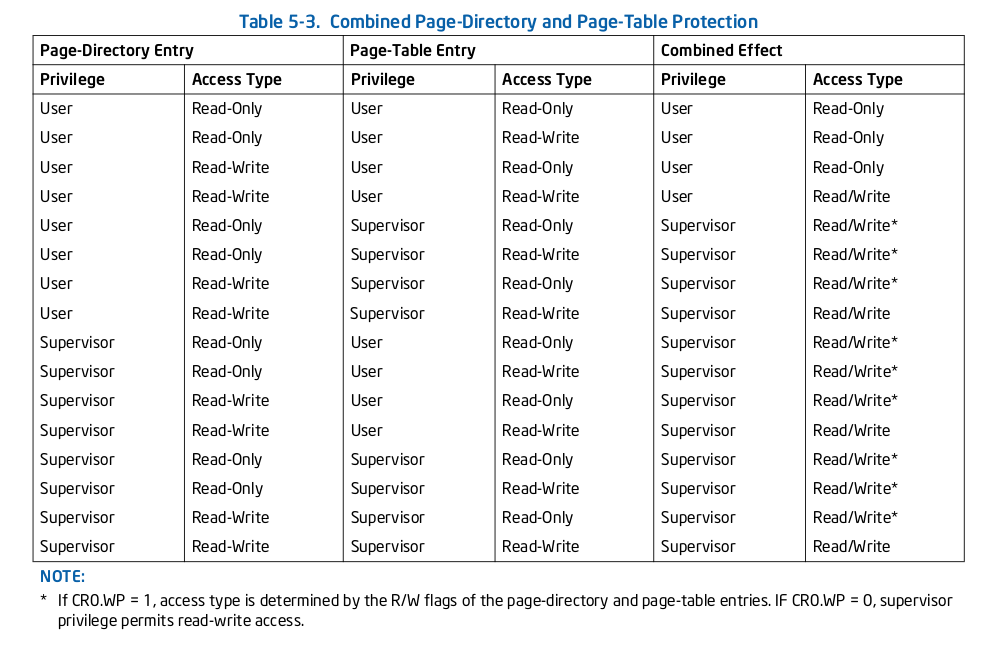
\includegraphics[height=10cm]{privilegios.png} 


\subsection{Pregunta 9: ¿Es posible desde dos directorios de página, referenciar a una misma tabla de páginas?}

Si, esto es posible ya que no hay restricciones al respecto. Cuando la unidad de paginación va al directorio de páginas lo que recupera es una dirección fisica alineada a $4Kb$ que le indica en que lugar de la memoria se encuentra el page table que buscamos, por lo que para lograr esto simplemente hay que asignarles la direccion de la tabla que se decea compartir en ambos directorios y listo.


\subsection{Pregunta 10: ¿Que es el TLB (Translation Lookaside Buffer) y para qué sirve?}cache de traducciones
La TLB es una cache de traducciones, en el mismo se guarda la dirección base de una pagina para obtener una direccion fisica más algunos bit de atributos necesarios, entre los cuales se encuentra LRU para saber cual es el próximo elemento de la TLB que debe ser desalojado en caso necesario.

Esto tiene su utilidad ya que se cuenta con el criterio de vecindad, el cual dice que si por ejemplo la dirección almacenada pertenece a una página de código, seguramente la proximas instrucciones estén en la misma página ahorrandose asi la traducción de las mismas que ya se pueden calcular a traves de la TLB. 


\subsection{Pregunta 11: ¿Qué pasa si en la interrupción de teclado no se lee la tecla presionada?}


\subsection{Pregunta 12: ¿Qué pasa si no se resetea el PIC?}


\subsection{Pregunta 13: Colocando un breakpoint luego de la cargar una tarea, ¿cómo se puede
verificar, utilizando el debugger de Bochs, que la tarea se cargó correctamente? ¿Cómo se
llega a esta conclusión?}


\subsection{Pregunta 14: ¿Cómo se puede verificar si la conmutación de tarea fue exitosa?}
Si la conmutación de la tarea fue exitosa, esta comenzará a ejecutarse, pudiendose ver en el debugger de Bochs su ejecución. Además de esto, es posible verificar, utilizando \textbf{info tss} si la TSS fue cargada correctamente observando los valores correspondientes a la tarea.


\subsection{Pregunta 15: Se sabe que las tareas llaman a la interrupción 0x80 y por 0x90. ¿Qué ocurre si esta no está implementada? ¿Por qué?}

Si estas interrupciones están definidas en la IDT pero no están implementadas, lo que ocurre es que el procesador empieza a ejecutar el código en la dirección especificada en la IDT entry correspondiente a la interrupción recibida. El resultado de esto es indeterminado, de acuerdo a lo que hayamos puesto en nuestro kernel en esa dirección de memoria.

Si en cambio las interrupciones no están definidas en la IDT, o la IDT entry correspondiente está mal definida (por ejemplo, si los campos segmento:offset apuntan a una dirección de memoria no definida) el procesador produce una excepción de protección general.

\end{document}